\documentclass[aps,prl,twocolumn,groupedaddress]{revtex4-1}
% \documentclass[aps,twocolumn,secnumarabic,balancelastpage,amsmath,amssymb,nofootinbib]{revtex4-1}
\usepackage{amsmath}
\usepackage{amssymb}
\usepackage{amsfonts}
\usepackage{color}
\usepackage{graphics}
\usepackage[pdftex]{graphicx}
\usepackage[utf8x]{inputenc}
\usepackage[colorlinks=true]{hyperref}

\newcommand{\ud}{\mathrm{d}}
\newcommand{\ue}{\mathrm{e}}
\newcommand{\ui}{\mathrm{i}}
\newcommand{\res}{\mathrm{Res}}
\newcommand{\Tr}{\mathrm{Tr}}
\newcommand{\dsum}{\displaystyle\sum}
\newcommand{\dprod}{\displaystyle\prod}
\newcommand{\dlim}{\displaystyle\lim}
\newcommand{\dint}{\displaystyle\int}
\newcommand{\fsno}[1]{{\!\not\!{#1}}}
\newcommand{\texp}[2]{\ensuremath{{#1}\times10^{#2}}}
\newcommand{\dexp}[2]{\ensuremath{{#1}\cdot10^{#2}}}
\newcommand{\eval}[2]{{\left.{#1}\right|_{#2}}}
\newcommand{\paren}[1]{{\left({#1}\right)}}
\newcommand{\lparen}[1]{{\left({#1}\right.}}
\newcommand{\rparen}[1]{{\left.{#1}\right)}}
\newcommand{\abs}[1]{{\left|{#1}\right|}}
\newcommand{\sqr}[1]{{\left[{#1}\right]}}
\newcommand{\crly}[1]{{\left\{{#1}\right\}}}
\newcommand{\angl}[1]{{\left\langle{#1}\right\rangle}}
\newcommand{\tpdiff}[4][{}]{{\paren{\frac{\partial^{#1} {#2}}{\partial {#3}{}^{#1}}}_{#4}}}
\newcommand{\tpsdiff}[4][{}]{{\paren{\frac{\partial^{#1}}{\partial {#3}{}^{#1}}{#2}}_{#4}}}
\newcommand{\pdiff}[3][{}]{{\frac{\partial^{#1} {#2}}{\partial {#3}{}^{#1}}}}
\newcommand{\diff}[3][{}]{{\frac{\ud^{#1} {#2}}{\ud {#3}{}^{#1}}}}
\newcommand{\psdiff}[3][{}]{{\frac{\partial^{#1}}{\partial {#3}{}^{#1}} {#2}}}
\newcommand{\sdiff}[3][{}]{{\frac{\ud^{#1}}{\ud {#3}{}^{#1}} {#2}}}
\newcommand{\tpddiff}[4][{}]{{\left(\dfrac{\partial^{#1} {#2}}{\partial {#3}{}^{#1}}\right)_{#4}}}
\newcommand{\tpsddiff}[4][{}]{{\paren{\dfrac{\partial^{#1}}{\partial {#3}{}^{#1}}{#2}}_{#4}}}
\newcommand{\pddiff}[3][{}]{{\dfrac{\partial^{#1} {#2}}{\partial {#3}{}^{#1}}}}
\newcommand{\ddiff}[3][{}]{{\dfrac{\ud^{#1} {#2}}{\ud {#3}{}^{#1}}}}
\newcommand{\psddiff}[3][{}]{{\frac{\partial^{#1}}{\partial{}^{#1} {#3}} {#2}}}
\newcommand{\sddiff}[3][{}]{{\frac{\ud^{#1}}{\ud {#3}{}^{#1}} {#2}}}

\begin{document}
\title{Motional Quantum Ground-State Cooing Outside the Lamb-Dicke Regime}
\author{Yichao Yu}
\author{Nicholas R. Hutzler}
\author{Jessie T. Zhang}
\author{Lee R. Liu}
\author{Kang-Kuen Ni}
\email{ni@chemistry.harvard.edu}
\affiliation{Department of Chemistry and Chemical Biology, Harvard University, Cambridge, Massachusetts, 02138, USA}
\affiliation{Department of Physics, Harvard University, Cambridge, Massachusetts, 02138, USA}
\affiliation{Harvard-MIT Center for Ultracold Atoms, Cambridge, Massachusetts, 02138, USA}

\date{\today}

\begin{abstract}
  Single neutral atom trapped in optical tweezer is a promising system for various applications
  in quantum information and simulation.
  The control of the motional states for such a system is crucial
  for exploiting its full potential.
  We report Raman sideband cooling of a single sodium atom to its three-dimensional
  motional ground state in an optical tweezer.
  Despite having a very large Lamb-Dicke parameter, high initial temperature and
  large differential AC Stark shift in the excited state,
  we achieved a ground state preparation fidelity of $77(4)\%$ after a few hundred ms of cooling
  by using a few new cooling techniques including addressing high order Raman sideband.
  We demonstrate that Raman sideband cooling to the 3D motional ground state is applicable to
  systems where tight confinement or low initial cooling is hard to achieve.
  The is particularly relevant for systems which are challenging to laser-cool,
  such as molecules and exotic atoms, and opens up a new approach for further cooling
  of these systems.
\end{abstract}

\maketitle

\begin{figure*}
  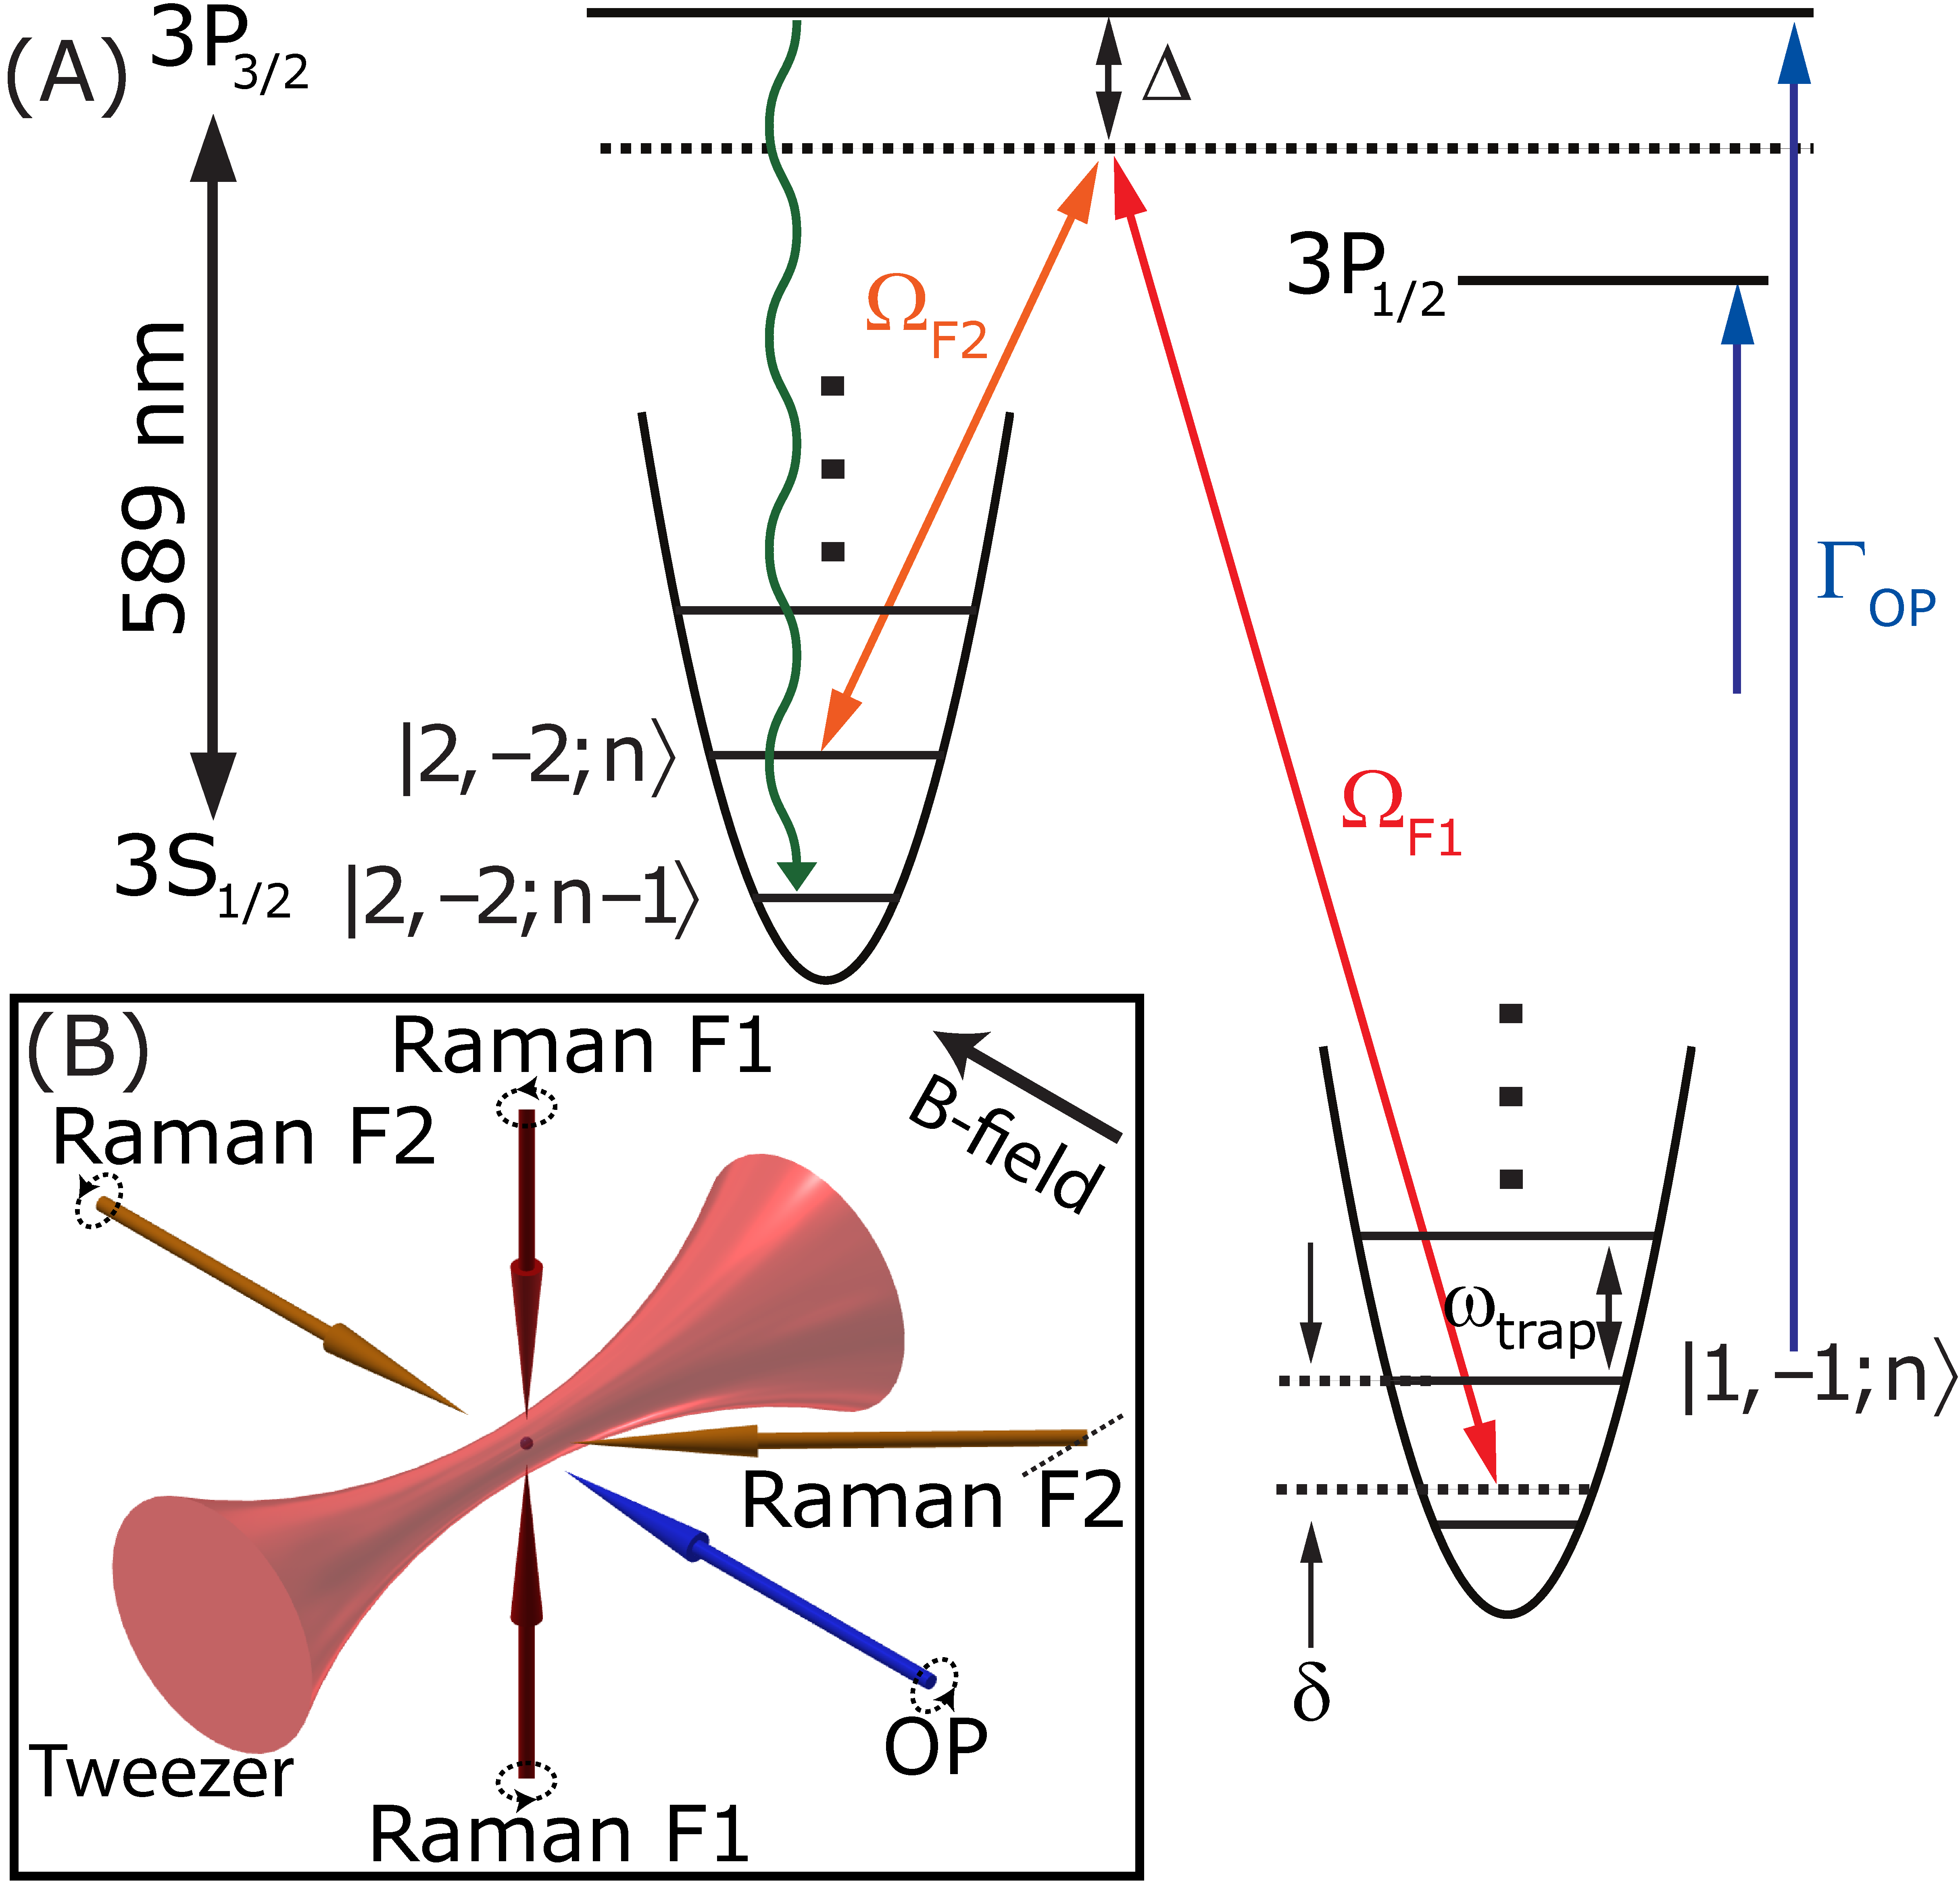
\includegraphics[height=5.2cm]{imgs/Na_RSC_schematic.pdf}
  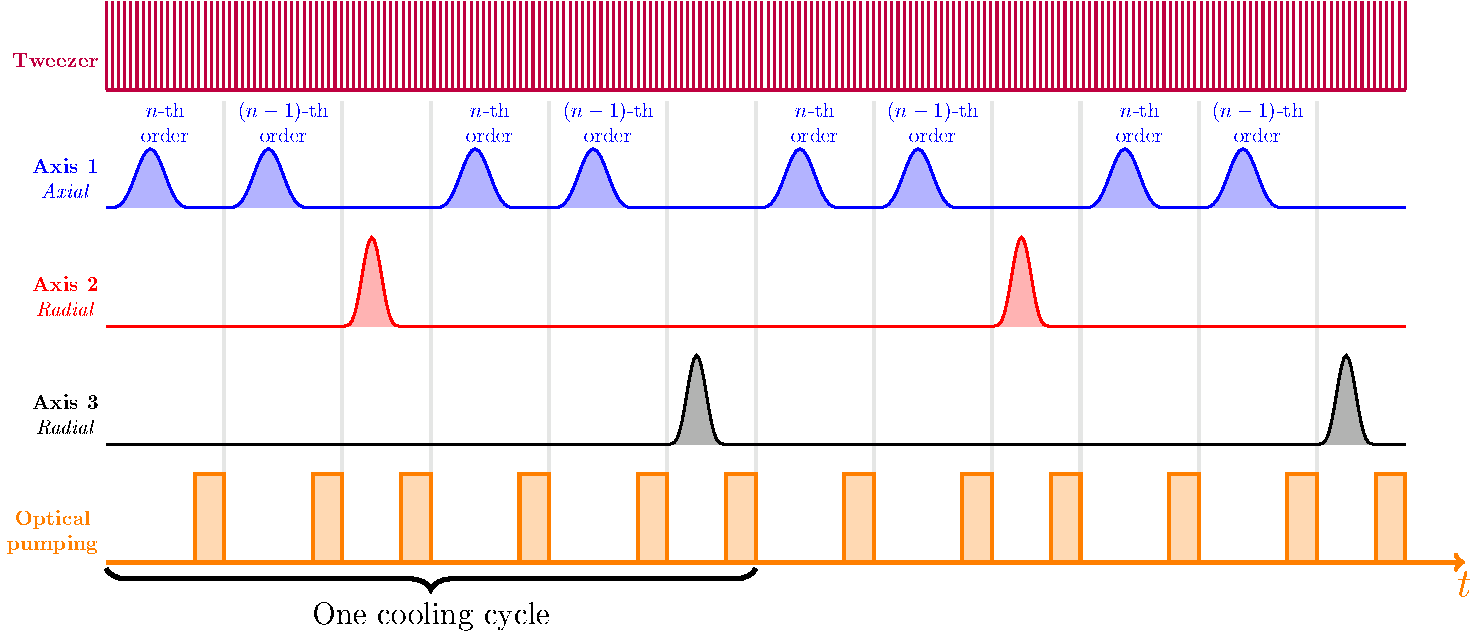
\includegraphics[height=4.5cm]{sequence.pdf}
  \caption{(A) Energy levels and schematic of Raman sideband cooling.
    The Raman transitions have a one photon detuning $\Delta=25$ GHz from the D2 line.
    We use D1 light with $\sigma^-$ polarization to repump atoms out of $|F=2,m_F=-1\rangle$
    state to minimize heating on the atom in $|F=2,m_F=-2\rangle$ state [TALK ABOUT THIS IN THE TEXT].
    (B) Geometry and polarizations of the Raman and optical pumping beams relative to the
    optical tweezer and bias magnetic field.
    (C) Schematic of the cooling sequence. The tweezer switches at 3 MHz to
    reduce light shifts during optical pumping. Each cooling cycle consists of $8$ pulses.
    The four axial pulses are addressing two neighboring cooling orders.
    The two pulses in each radial directions are either addressing two neighboring cooling orders
    or having different length on the first order when most of the population are below $n=3$
    towards then end of the cooling sequence.
    \label{f-setup}}
\end{figure*}
\begin{figure}[b]
  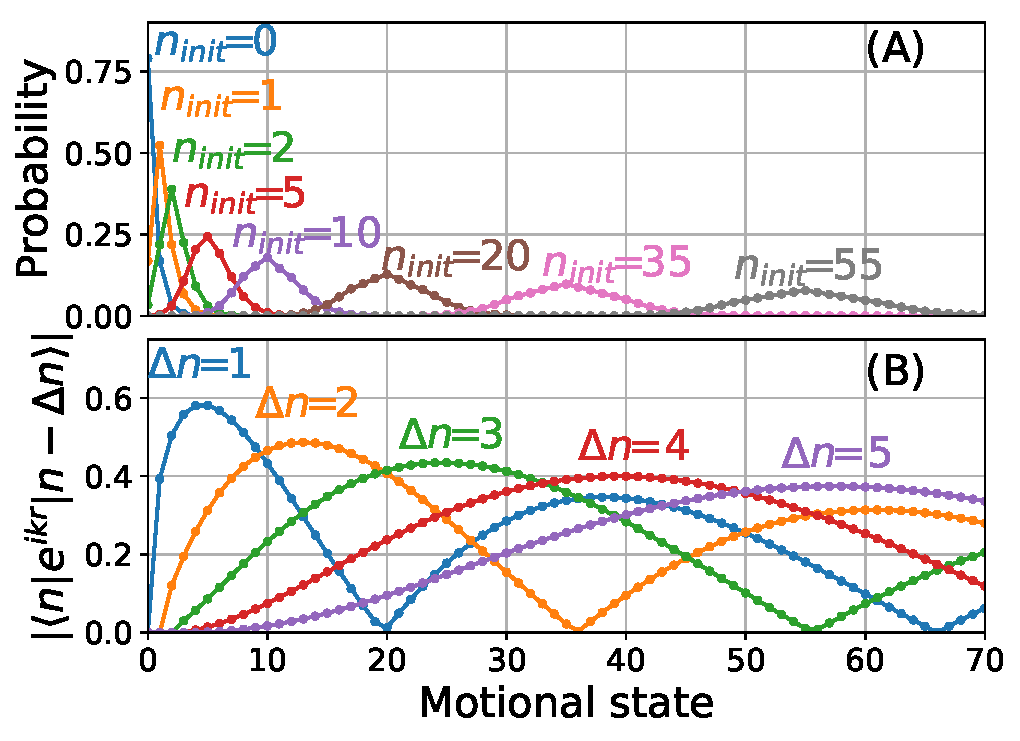
\includegraphics[width=8.5cm]{imgs/fig2_raman_op.pdf}
  \caption{Matrix elements and heating probabilities as a function of motional state.
    The range plotted covers $99\%$ of the initial thermal distribution.
    (A) Matrix elements for Raman transition in the axial direction showing deviation from
    $\sqrt{n}$ scaling and multiple minimums for different sideband orders.
    (B) Heating probability during the optical pumping step for all three axis.
    Due to the large Lamb-Dicke parameter,
    there is a high probability of heating especially in the axial direction.
    \label{f-ld}}
\end{figure}
\begin{figure*}
  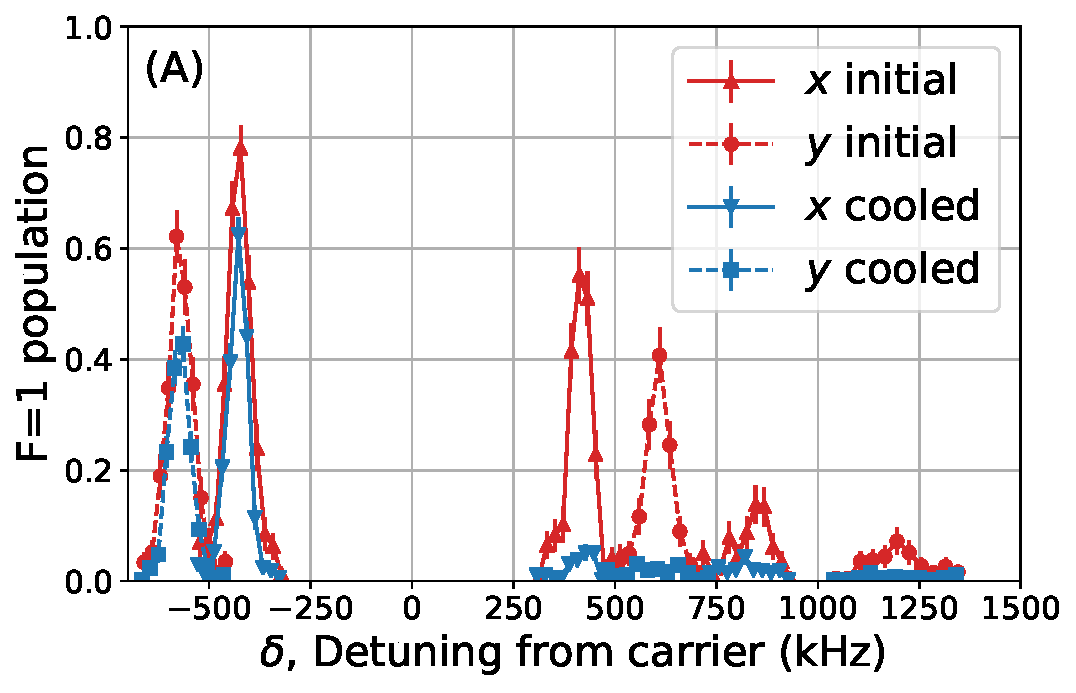
\includegraphics[height=4.2cm]{imgs/spectrum_r.pdf}
  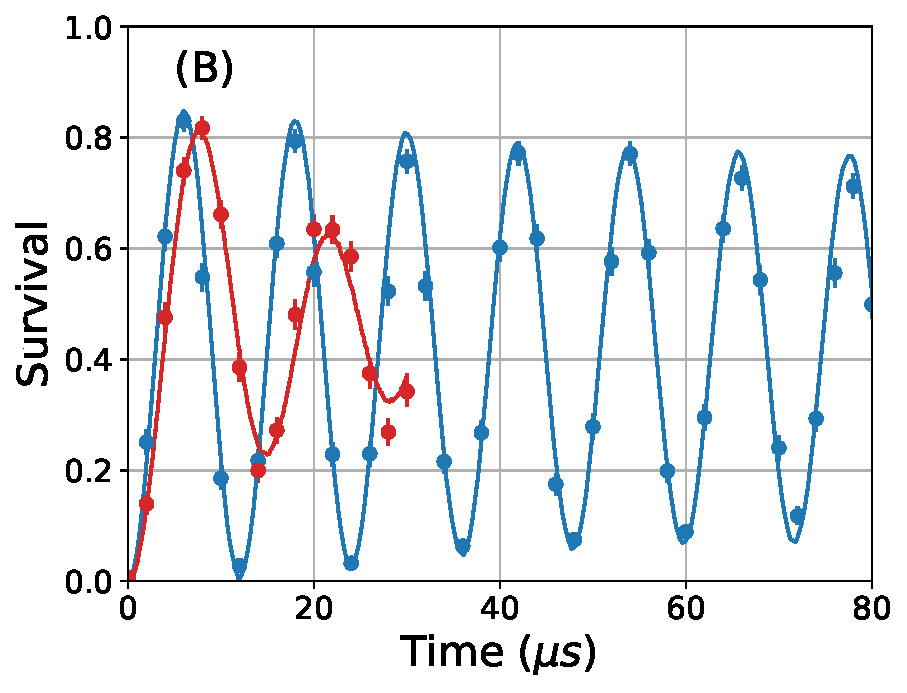
\includegraphics[height=4.2cm]{imgs/rabi_flop_r3_0.pdf}
  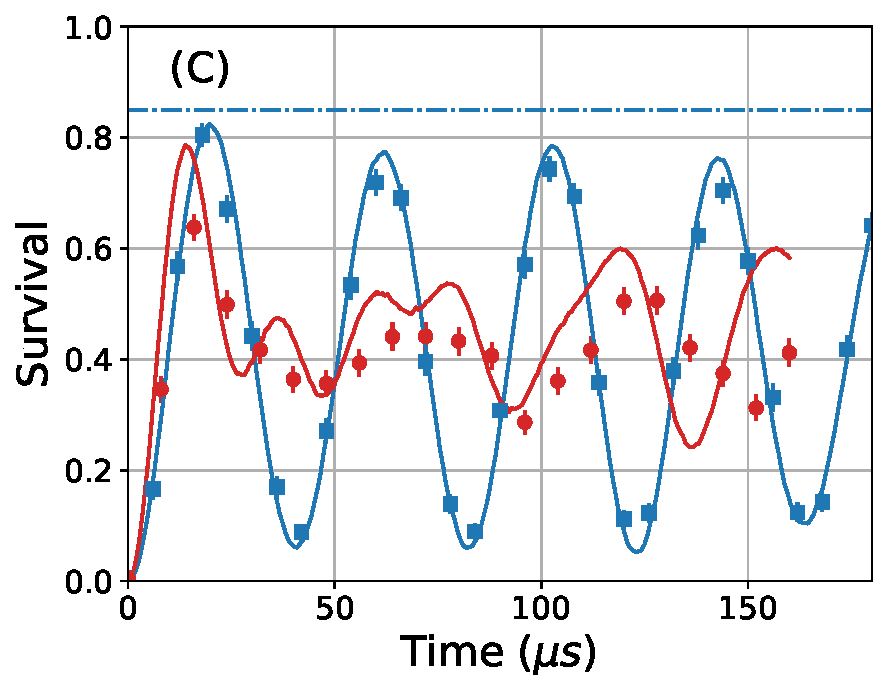
\includegraphics[height=4.2cm]{imgs/rabi_flop_r3_p1.pdf}
  \caption{Radial Raman sideband spectrum of first order heating, first order cooling and
    second order cooling (A) before and (B) after Raman sideband cooling.
    Rabi flopping on axis 3 (C) carrier and (D) first order heating sideband
    after cooling.
    Solid lines in (C) and (D) are theoretical fit with a ground state probability of $93\%$.
    \label{f-radial}}
\end{figure*}
\begin{figure*}
  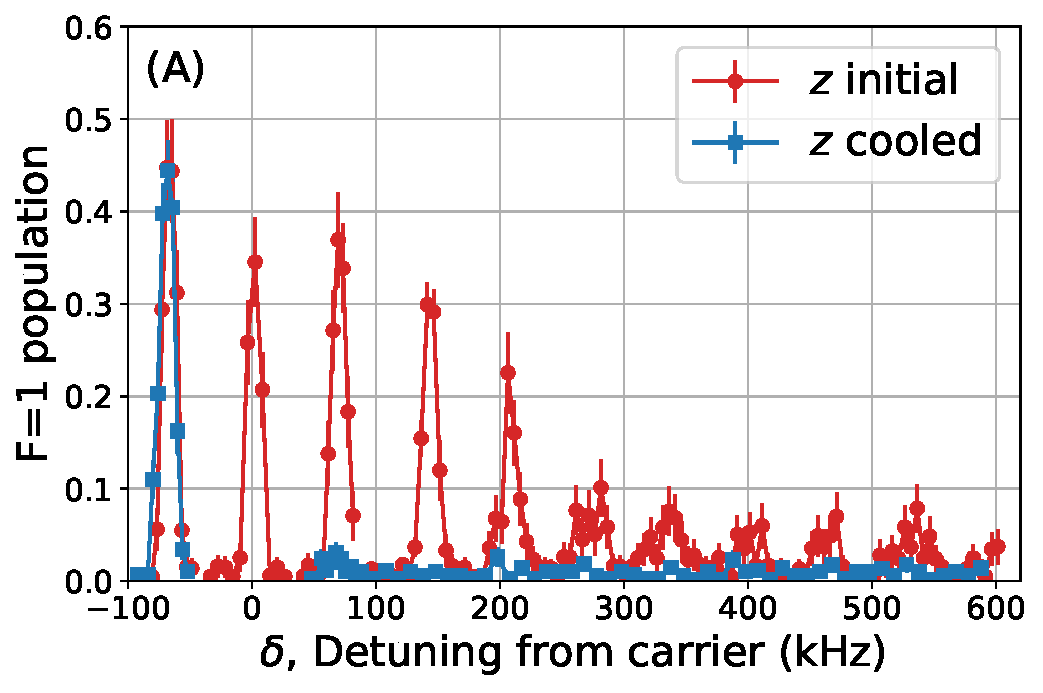
\includegraphics[height=4.2cm]{imgs/spectrum_a1.pdf}
  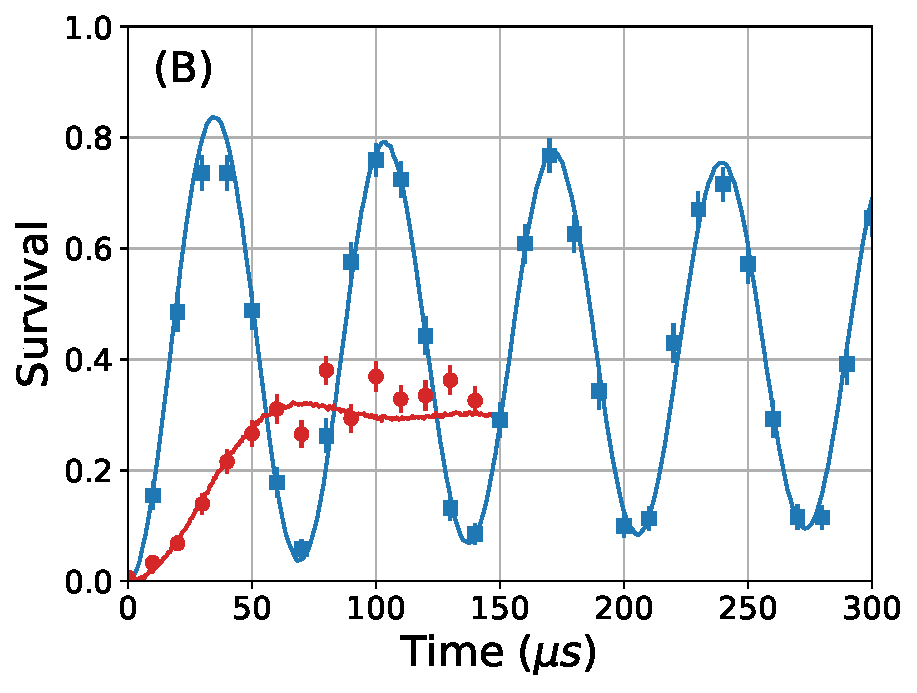
\includegraphics[height=4.2cm]{imgs/rabi_flop_a1_0.pdf}
  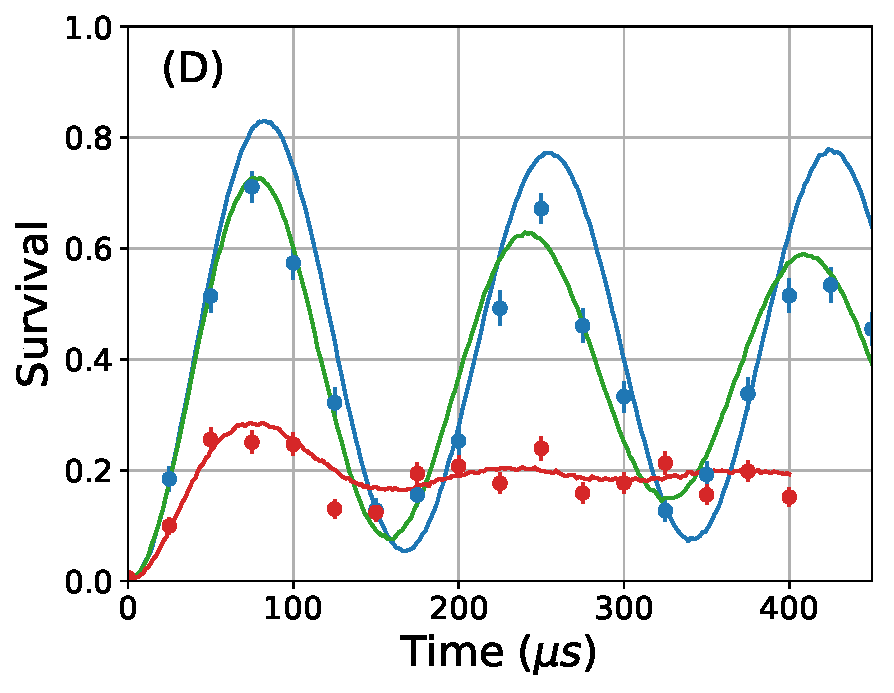
\includegraphics[height=4.2cm]{imgs/rabi_flop_a1_p1.pdf}
  \caption{Axial Raman sideband spectrum from first order heating to eighth order cooling
    (A) before and (B) after Raman sideband cooling.
    The data for the second and higher orders of cooling sidebands are taken with 150 $\mu$s
    pulse time and the rest are taken with 125 $\mu$s pulse time.
    Rabi flopping on axial (C) carrier and (D) first order heating sideband
    after cooling.
    Solid lines in (C) and (D) are theoretical fit with a ground state probability of $92\%$.
    \label{f-axial}}
\end{figure*}

Systems of single neutral atoms trapped in optical tweezers are an exciting platform to study quantum information, quantum chemistry,
and quantum simulation of many-body systems [REF].
This approach provides full single-site resolution and control, and can feature long-range interactions via Rydberg atoms,
polar molecules, or dipolar atoms [REF].
Polar molecules in particular offer the additional advantages of long-lived internal states and a high degree of tunability,
including the shape, range, and strength of the interaction [REF].
Optical tweezers can also be re-arranged in real-time, allowing rapid preparation of atoms in complex geometries with high fidelity [REF].

In order to achieve long coherence times and full quantum control of the system,
it is typically necessary to cool the atom to the
three dimensional motional ground state in the optical tweezer.
This has been demonstrated for neutral Rb\cite{Thompson2013,Kaufman2012} and Cs [REF] in experiments that had low initial temperature and small Lamb-Dicke parameter.
These features
may not be easily achievable for other systems, such as directly laser-cooled polar molecules [REF],
or atoms with challenging sub-Doppler cooling such as Na, K, and Li [REF].
In this letter, we cool single sodium atoms
trapped in optical tweezers to the motional ground state with Raman sideband cooling.
Despite having a large Lamb-Dicke parameter and high initial temperature, we are able to achieve a ground state probability of $77(4)\%$
by utilizing several new cooling techniques and a carefully optimized cooling sequence.  Our approach is quite general, and opens up ground-state cooling for other systems.

As mentioned previously, in order to perform Raman sideband cooling efficiently and
minimize the heating during the optical pumping, we need to have a low initial temperature and
a small Lamb-Dicke parameter. However, since the Lamb-Dicke parameter $\eta$ is inversely
proportional to $\sqrt[4]{m}/\lambda$ where $m$ is the mass of the atom and $\lambda$
is the wavelength of the atomic transition,
it is larger for sodium given the same trap depth due to its low mass and short D line wavelength.
With 45 mW of power in the trap, we measure trapping frequencies of
$\{\omega_1,\omega_2,\omega_3\}/2\pi = \{69, 430, 590\}\ \text{\text{kHz}}$ [ERROR BARS]
which corresponds to optical pumping Lamb-Dicke parameters of
$\{\eta^{OP}_1,\eta^{OP}_2,\eta^{OP}_3\} = \{0.60, 0.24, 0.21\}$ [ERROR BARS].
Moreover, due to the small hyperfine structure in the $3^2P_{3/2}$ manifold,
the sub-Doppler cooling in sodium is also less efficient and we start the
Raman sideband cooling with a initial temperature of 70 $\mu$K. Combined with the high Lamb-Dicke
parameters, this gives us a initial effective optical pumping Lamb-Dicke parameters of
$\{\eta^{OP}_{1eff},\eta^{OP}_{2eff},\eta^{OP}_{3eff}\} = \{3.97, 0.67, 0.50\}$
As a result, there is a very high probability of heating during the optical pumping step
(figure \ref{f-ld}B) causing an estimated $30\%$ average heating probability during optical pumping
in the weakly confined axial direction.

Fortunately, the high Lamb-Dicke parameters also
provide us with tools to overcome this issue. The Lamb-Dicke parameters for the
Raman transitions in our configuration are $\{\eta^R_{1},\eta^R_{2},\eta^R_{3}\} = \{0.40, 0.34, 0.29\}$. As shown in
figure \ref{f-ld}A, the high Raman Lamb-Dicke parameters causes a strong coupling to higher orders
of cooling sidebands, especially for high motional states.
This enables cooling of atoms in high motional states by driving higher order Raman sidebands,
removing more motional energy in a single cooling pulse and offsetting the effect of heating. Since the heating probability is higher for high motional states,
cooling on these high order sidebands can greatly suppress the high heating during
optical pumping during the initial cooling. Since the coupling strength of different orders
do not reach their minimums at the same time [FIG], using multiple orders of motional sidebands
for cooling also avoids accumulation of population near the coupling minimum of a particular
order, which improves the overall efficiency of the cooling process.

The high initial temperature also causes additional complications.  First, population in high motional states means that the atoms sample
the anharmonicity of the trap away from the harmonic center.  This results in sidebands that are broader and of reduced height [FIG], and limits the Rabi frequency of the Raman pulse
on the radial sidebands to be no lower than tens of kHz in order to drive atoms in
different motional states equally.  [EXPLAIN THIS A LITTLE MORE].
Second, the deep trap that is needed to trap and image single sodium atom also creates
a very large AC Stark shift in the excited state (as large as 300 MHz).
This creates large, position-dependent detuning for the optical pumping light and mixes the excited state state hyperfine levels,
which affects the branching ratios and increases the number of photons needed for optical pumping.
We solve this issue by switching the trapping light at $3\text{MHz}$
during the whole cooling sequence, similar to our loading and imaging process \cite{Hutzler2017-LightShifts}, but leave on the OP light with constant intensity.
Due to the large light shift, the OP light is effectively off when the trap light is on.
Since the atom can only be addressed by the optical pumping light when the trap light is off,
the effect of light shift on optical pumping fidelity is suppressed.

Taking all these features of our system into account, we use a Monte-Carlo simulation to verify
the validity of our method [WRITE BRIEF SUMMARY IN APPENDIX?].
In the simulation, we can observe the high heating rate due to the high Lamb-Dicke parameters
and confirm that by using high order Raman sideband transition in the cooling sequence we can
suppress this effect and reduces the motional energy of the atom faster.
The simulation is also used to guide the optimization of the cooling sequence by exploring the
large parameter space and finding a robust cooling strategy. As shown in figure \ref{f-setup}B,
we found that instead of cooling on only one sideband order at a time, it is generally more
efficient to alternate the cooling pulse between two neighboring orders (axial) or pulse lengths.
A cooling sequence like this minimizes the accumulation of atom in a state not addressed by a
particular Raman pulse parameter.

For the more tightly confined radial directions,
we begin the cooling with $\{\bar n_2, \bar n_3\}=2.2, 1.9$ [ERROR BARS].
The radial sideband spectra of the initial distribution is shown in figure \ref{f-radial}A
where we can clearly see the first order heating, first order cooling and
second order cooling sidebands.
After applying around 1000 cooling pulses cooling in all three dimensions
starting with cooling on the radial second order,
the Raman spectrum with the same parameters is shown in figure \ref{f-radial}B,
where the first and second order cooling sidebands on both axis are suppressed.
Given the absence of the second order cooling sideband,
we can estimate the ground state probability in each direction based on the height of
the first order cooling and heating sideband to be $90(2)\%$ and $94(3)\%$.

It is important to note that the large Raman Lamb-Dicke parameters $\eta^R$ mean that we must use caution when measuring the temperature.
Traditional sideband thermometry uses
the ratio of the cooling and heating sidebands to measure $\bar n / (\bar n + 1)$, which relies
on the coupling strength to be proportional to $\sqrt{n}$. However, outside the
Lamb-Dicke regime, the coupling strength deviates from this simple scaling rule rapidly as
shown in figure \ref{f-ld}A.
When the atom temperature is still high,
we measure the heights of multiple sidebands to make sure no population is hidden at the
minimum of one sideband order. Once the atom is cooled down, we estimate the temperature
and ground state population under the assumption that only a few states are populated.
We can verify the result via an independent measurement of Rabi flopping on the carrier and heating
sidebands. This data is shown before and after cooling in Figures
\ref{f-radial}C and \ref{f-radial}D
and yields $90\%$ and $92\%$ [ERROR BARS],
showing good agreement between the two methods.

The axial direction is much less confined and therefore has a much higher initial effective
Lamb-Dicke parameter of $\eta^{OP}_{eff1}\approx 3.97$, and is therefore more difficult to cool.
Figure \ref{f-axial}A shows the Raman spectrum in the axial direction
before applying Raman sideband cooling; the clearly resolved sidebands
up to eighth order indicates population in highly-excited motional levels.
Therefore, we begin our cooling sequence by driving Raman transitions on the eighth order axial
cooling sideband. After applying the cooling sequence identical to the one we use to cool
the radial directions, the spectrum is shown in figure \ref{f-axial}B.
All of the high order ($\geqslant2$) axial cooling sidebands disappear, and the first order
cooling sideband is strongly suppressed.
The ground state probability calculated from this spectrum is $92(3)\%$.
We can again use Rabi flopping on the carrier and heating sideband to verify this result
similar to the radial direction. In this case, we see very good agreement on the carrier
(figure \ref{f-axial}B) but there is additional decoherence on the axial first order
heating sideband (figure \ref{f-axial}C).
We believe this decoherence is caused by technical noise, which is the most pronounced
on this transition due to its slow Rabi frequency.
The decoherence time scale is consistent with magnetic field fluctuations of XXX mG that we have measured in the lab, which produces
a Zeeman shift of around $5\text{kHz}$.


Combining the axial and radial cooling results,
we have achieved a 3D ground state probability of $77(4)\%$.
We believe this is currently limited by off-resonant scattering from the Raman beams
and the resonance shift caused by magnetic field fluctuations.
Improvements on these [HOW?] should improve the cooling performance even further.
We have shown that despite the difficulty in cooling sodium atoms,
it is possible to achieve reliable three dimensional cooling with significant ground state
probability using new cooling techniques and a optimized cooling sequence.
This opens up the possibility of cooling a large variety of systems to their motional ground
state using Raman sideband cooling that is challenging to laser cool
including molecules and exotic atoms.

% Missing:
% ?? Blackman pulse vs square pulse

\bibliography{paper}
\end{document}
